\begin{figure*}[t]
\centering
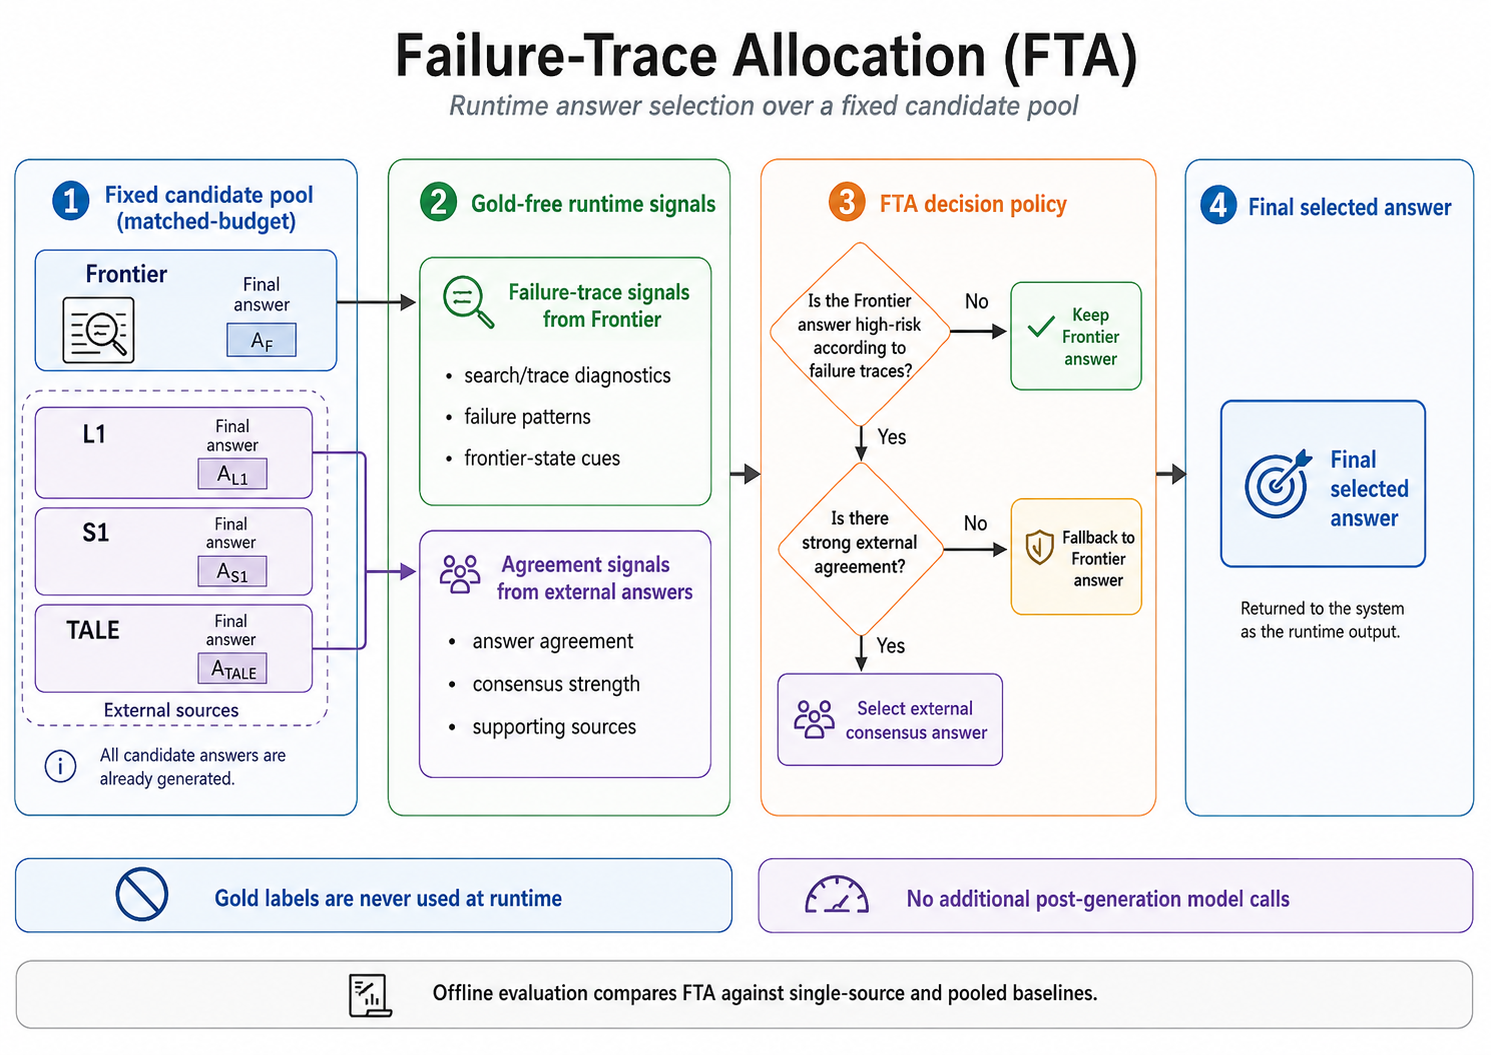
\includegraphics[width=0.98\textwidth]{figures/figure1_fta_method_overview.png}
\caption{%
  Failure-Trace Allocator (FTA) decision pipeline.
  Step~1: a fixed candidate pool is pre-generated at matched budget
  (Frontier, L1, S1, TALE; all candidate answers are generated before
  runtime selection begins).
  Step~2: gold-free runtime signals are derived from the frontier trace
  (failure diagnostics, failure patterns, frontier-state cues) and from
  agreement signals across external answers.
  Step~3: the FTA decision policy applies the two-gate logic described in
  Section~\ref{sec:method}: the Low-Depth Guard (LDG) checks for a
  structurally weak frontier trace; the External-Consensus Fallback (ECO)
  checks for unanimous external disagreement with the frontier answer.
  Step~4: the selected answer is returned as the runtime output.
  Gold labels are never used at runtime;
  no additional post-generation model calls are issued.
  Offline evaluation compares FTA against single-source and pooled baselines.
}
\label{fig:method_overview}
\end{figure*}
